\documentclass{article}

% Language setting
% Replace `english' with e.g. `spanish' to change the document language
\usepackage[english]{babel}

% Set page size and margins
% Replace `letterpaper' with `a4paper' for UK/EU standard size
\usepackage[letterpaper,top=2cm,bottom=2cm,left=3cm,right=3cm,marginparwidth=1.75cm]{geometry}

% Useful packages
\usepackage{amsmath}
\usepackage{graphicx}
\usepackage[colorlinks=true, allcolors=blue]{hyperref}
\usepackage{caption}
\usepackage{subcaption}

\title{TP4 - Programmation 3D}
\author{Beldjilali Maxime}

\begin{document}
\maketitle

\section{Bilan}

J'ai eu des difficultés à comprendre la base de code fournis et dans le niveau 1 il n'était pas clair qu'il fallait rajouter un éclairage. Cependant le sujet était intéressant et les résultats satisfaisants.

\section{Niveau 0}

\begin{figure}[h]
    \centering
    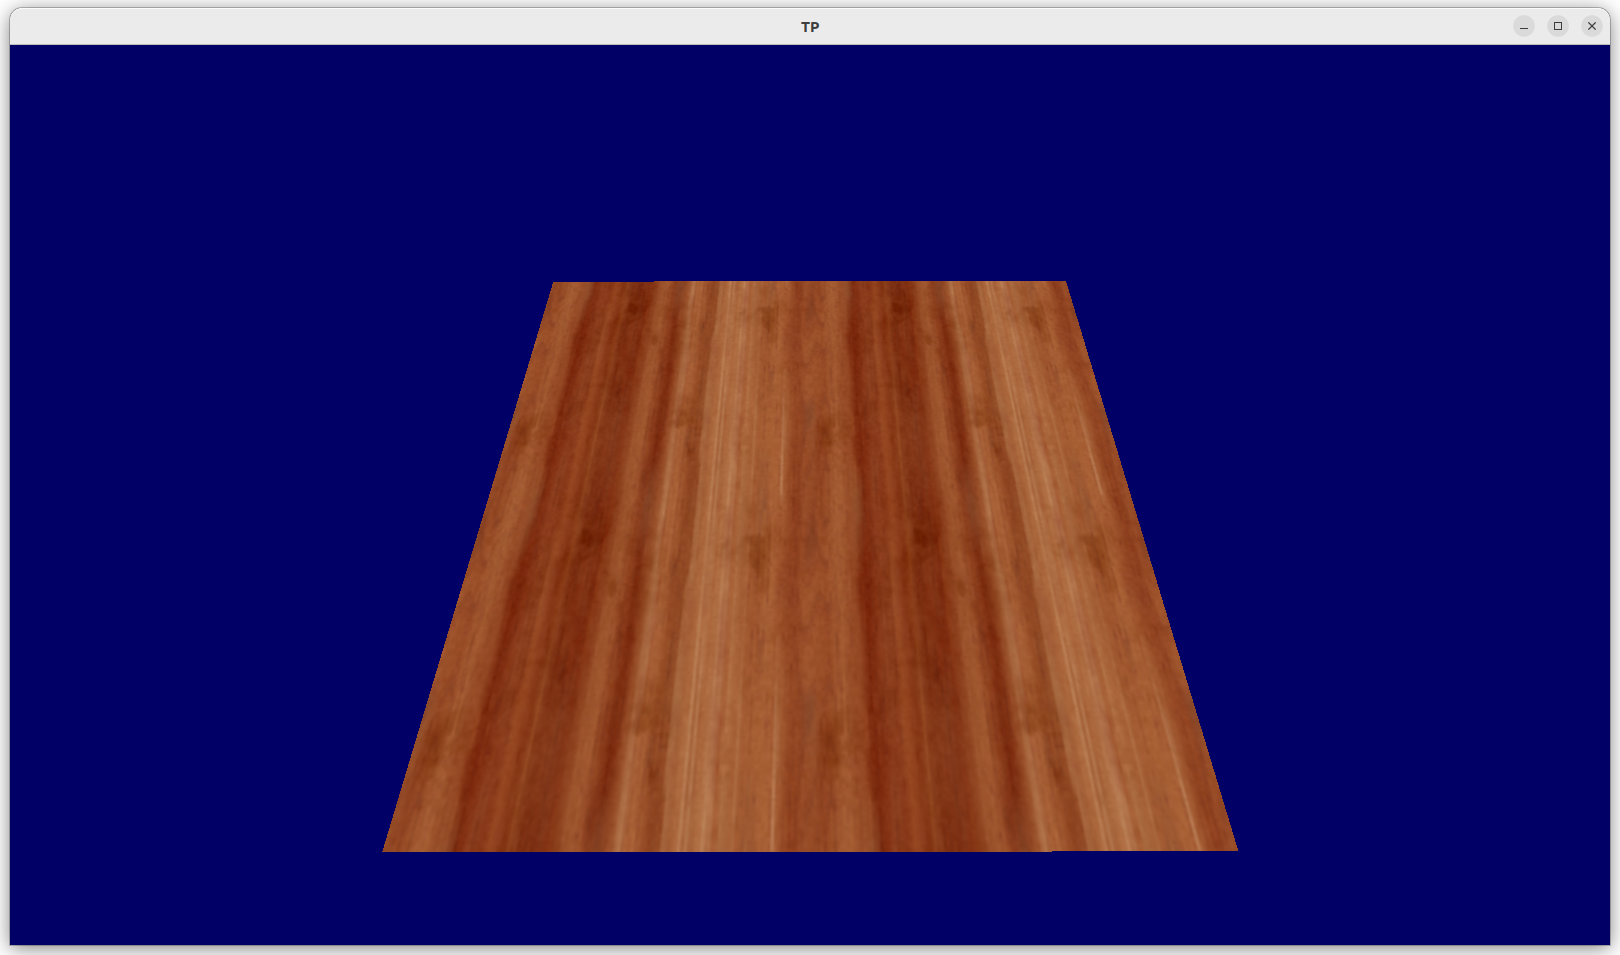
\includegraphics[width=0.5\linewidth]{images/placageTexture.png}
    \caption{Plaquage d'une texture 2D}
    \label{fig:plaquageTexture}
\end{figure}

\section{Niveau 1}

\begin{figure}[h]
    \centering
    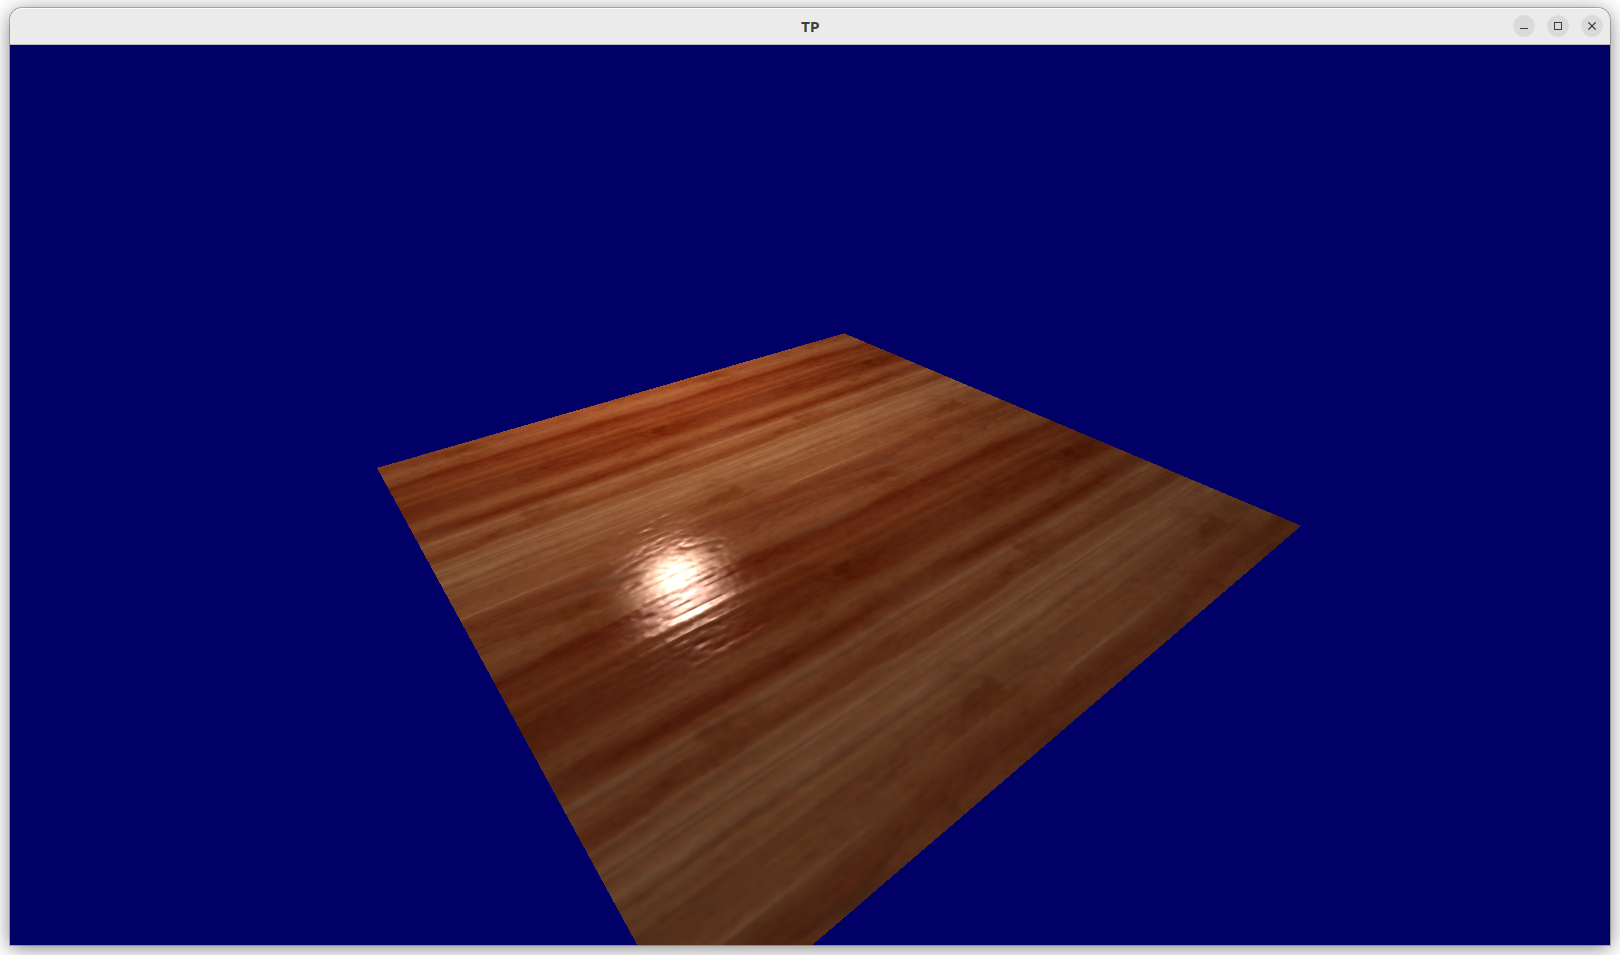
\includegraphics[width=0.5\linewidth]{images/normalMapping.png}
    \caption{Normal mapping}
    \label{fig:normalMapping}
\end{figure}

\newpage

\section{Niveau 2}

\begin{figure}[h]
    \centering
    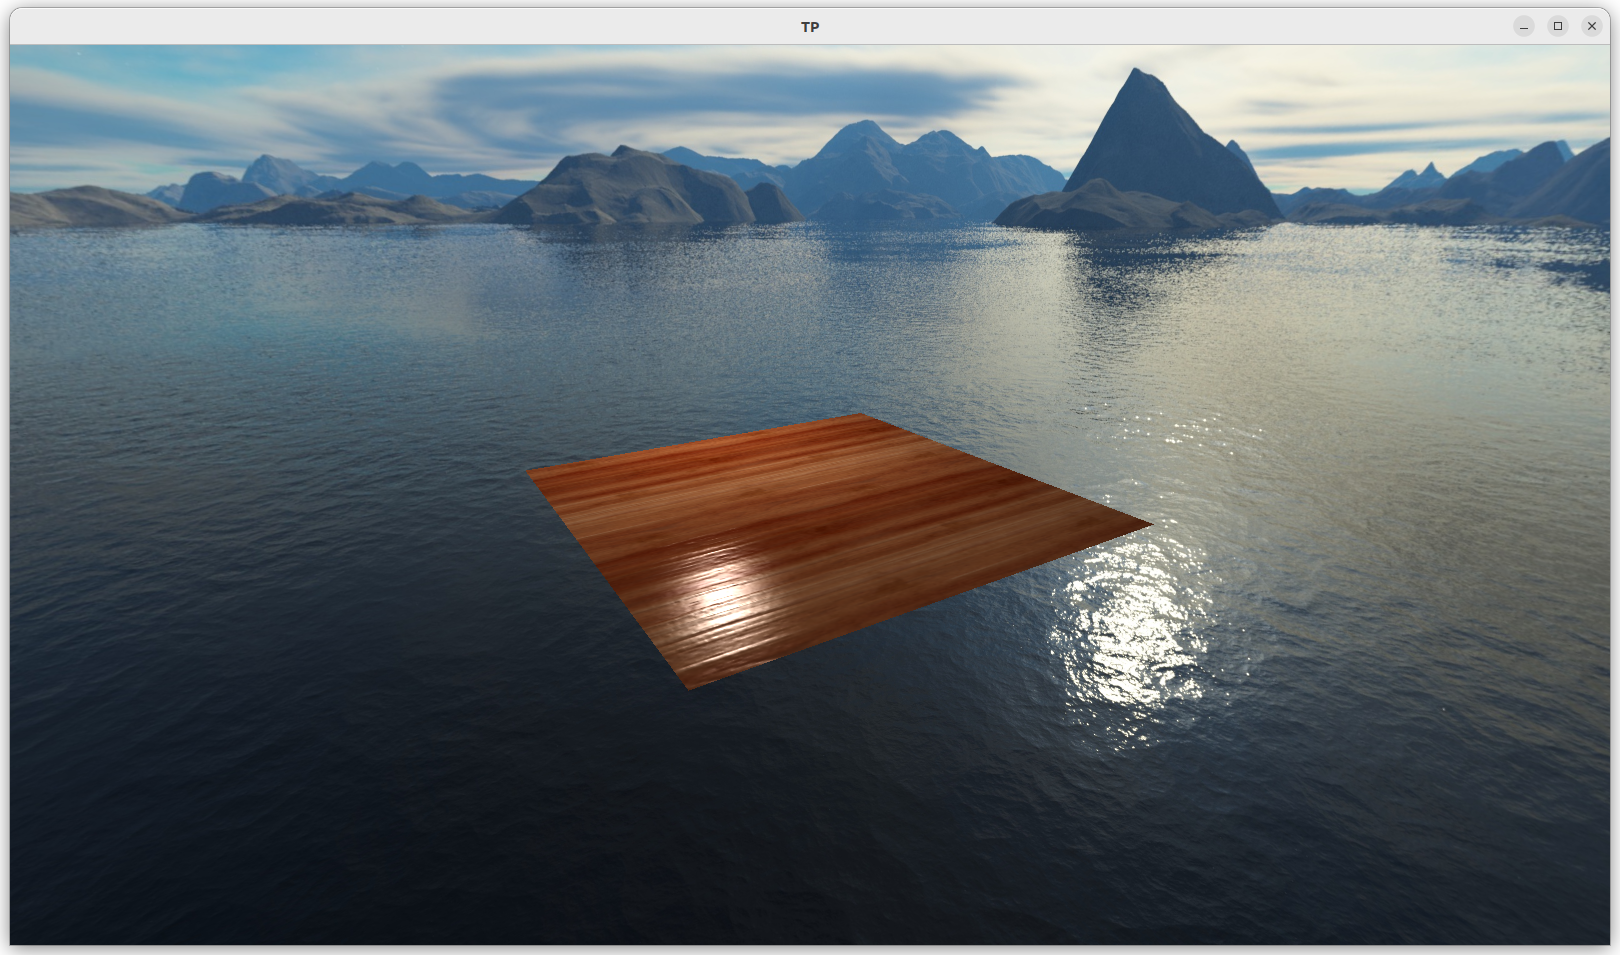
\includegraphics[width=0.5\linewidth]{images/skybox.png}
    \caption{Skybox}
    \label{fig:skybox}
\end{figure}

\begin{figure}[h]
     \centering
     \begin{subfigure}[b]{0.49\textwidth}
         \centering
         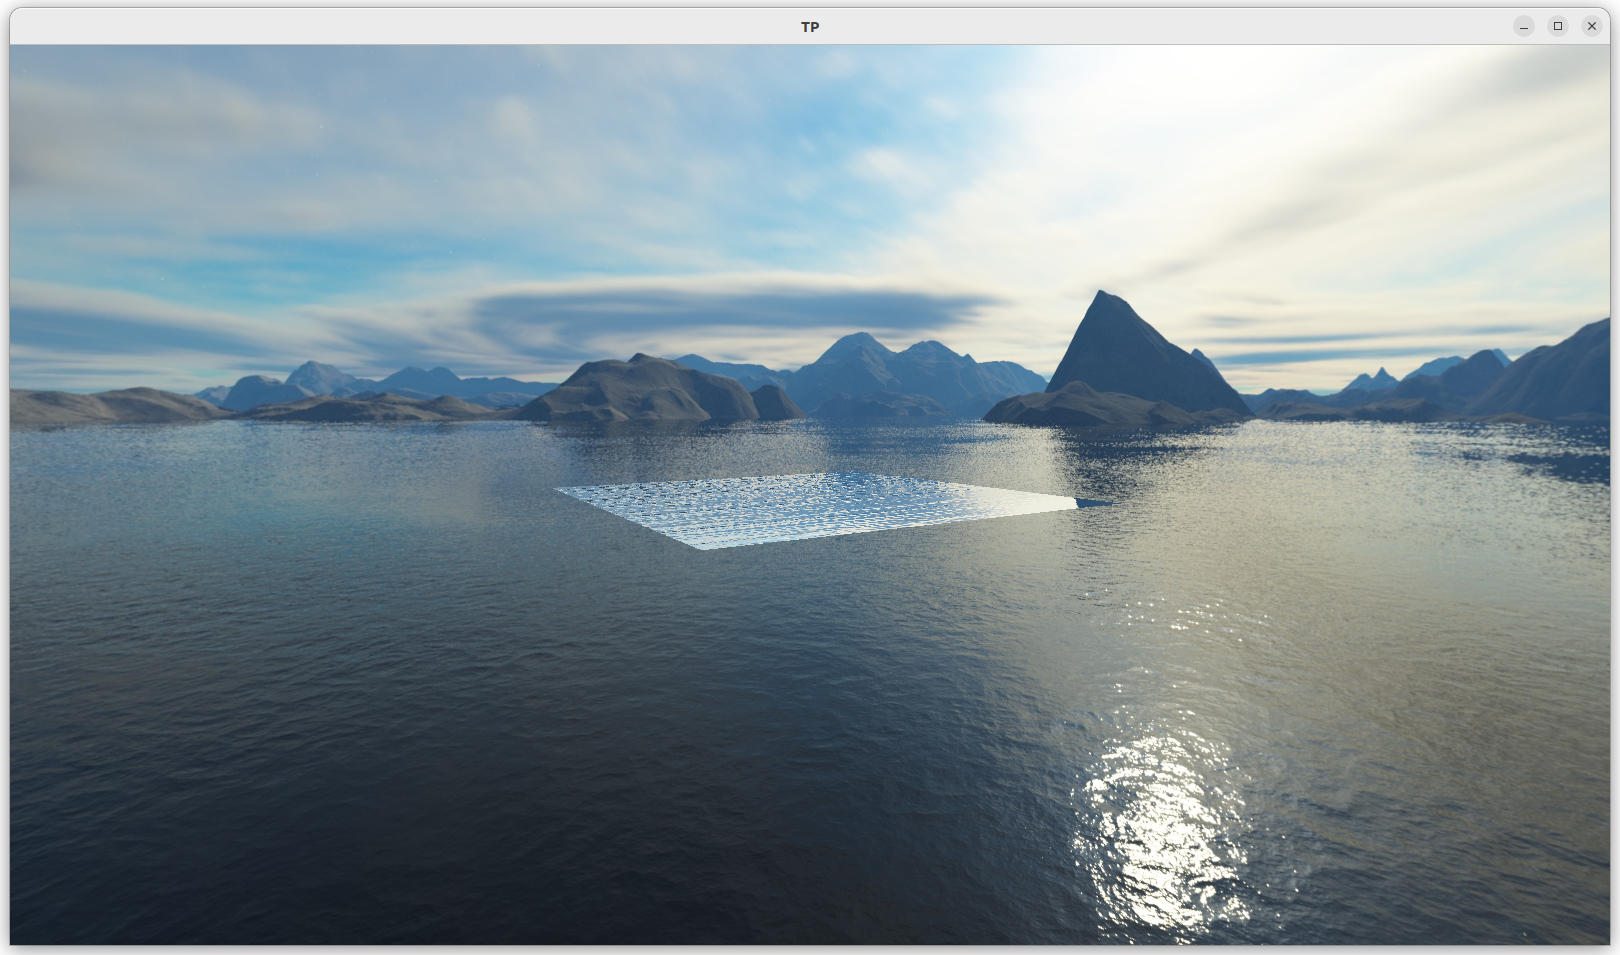
\includegraphics[width=\textwidth]{images/renduReflectif1.png}
     \end{subfigure}
     \hfill
     \begin{subfigure}[b]{0.49\textwidth}
         \centering
         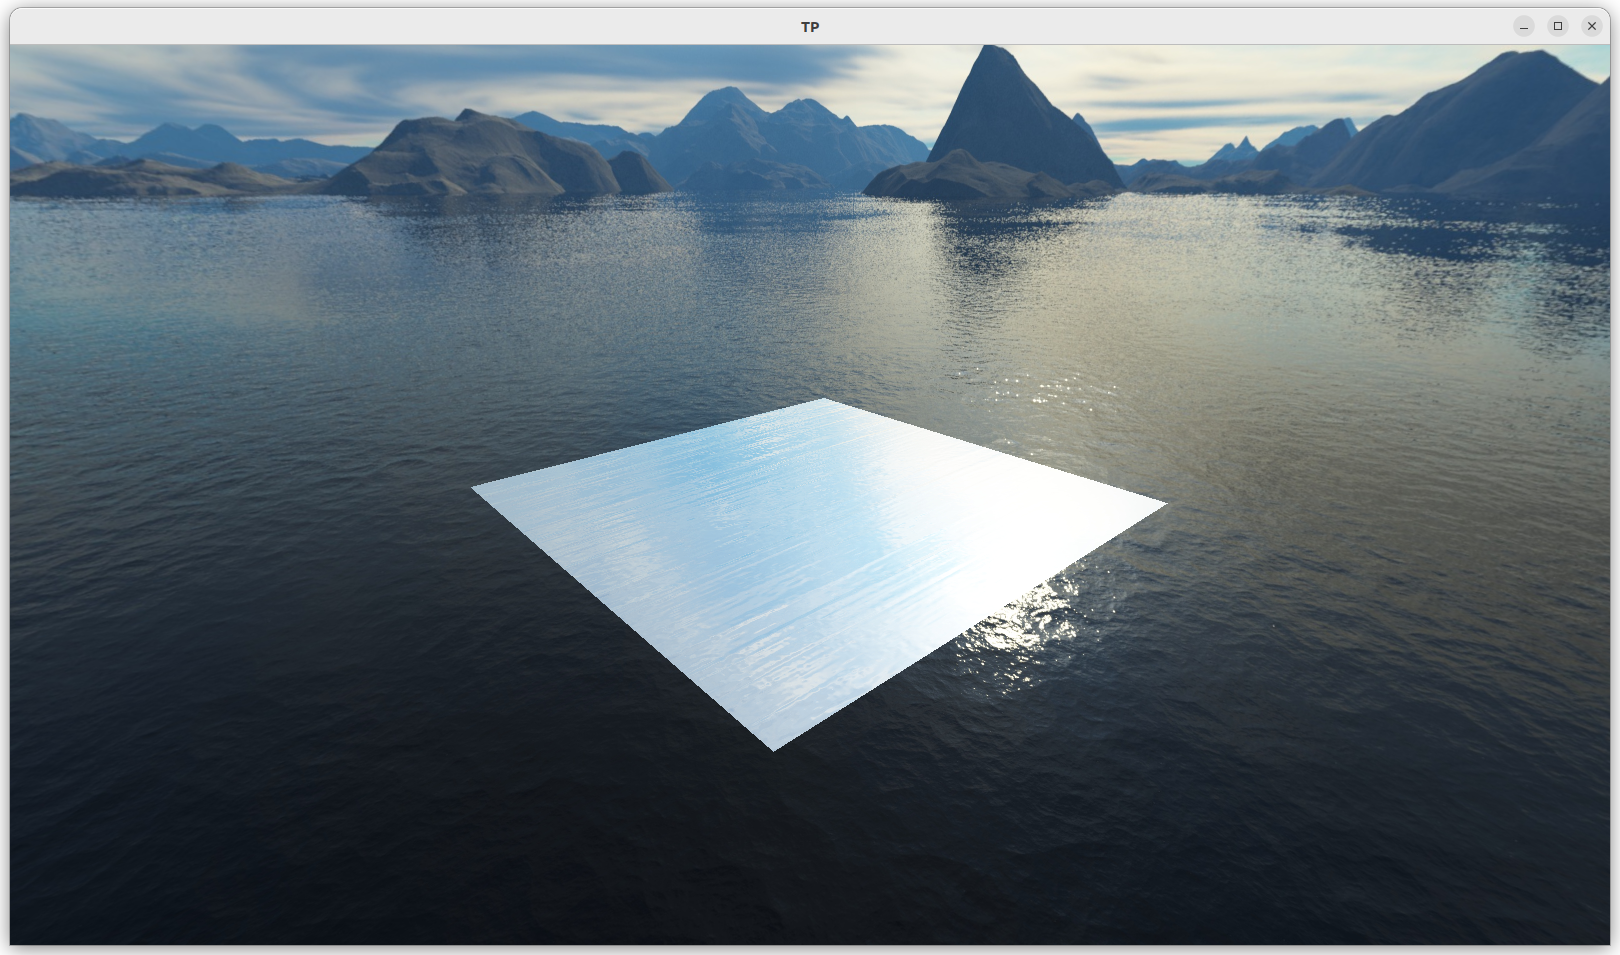
\includegraphics[width=\textwidth]{images/renduReflectif2.png}
     \end{subfigure}
     \hfill
     \begin{subfigure}[b]{0.49\textwidth}
         \centering
         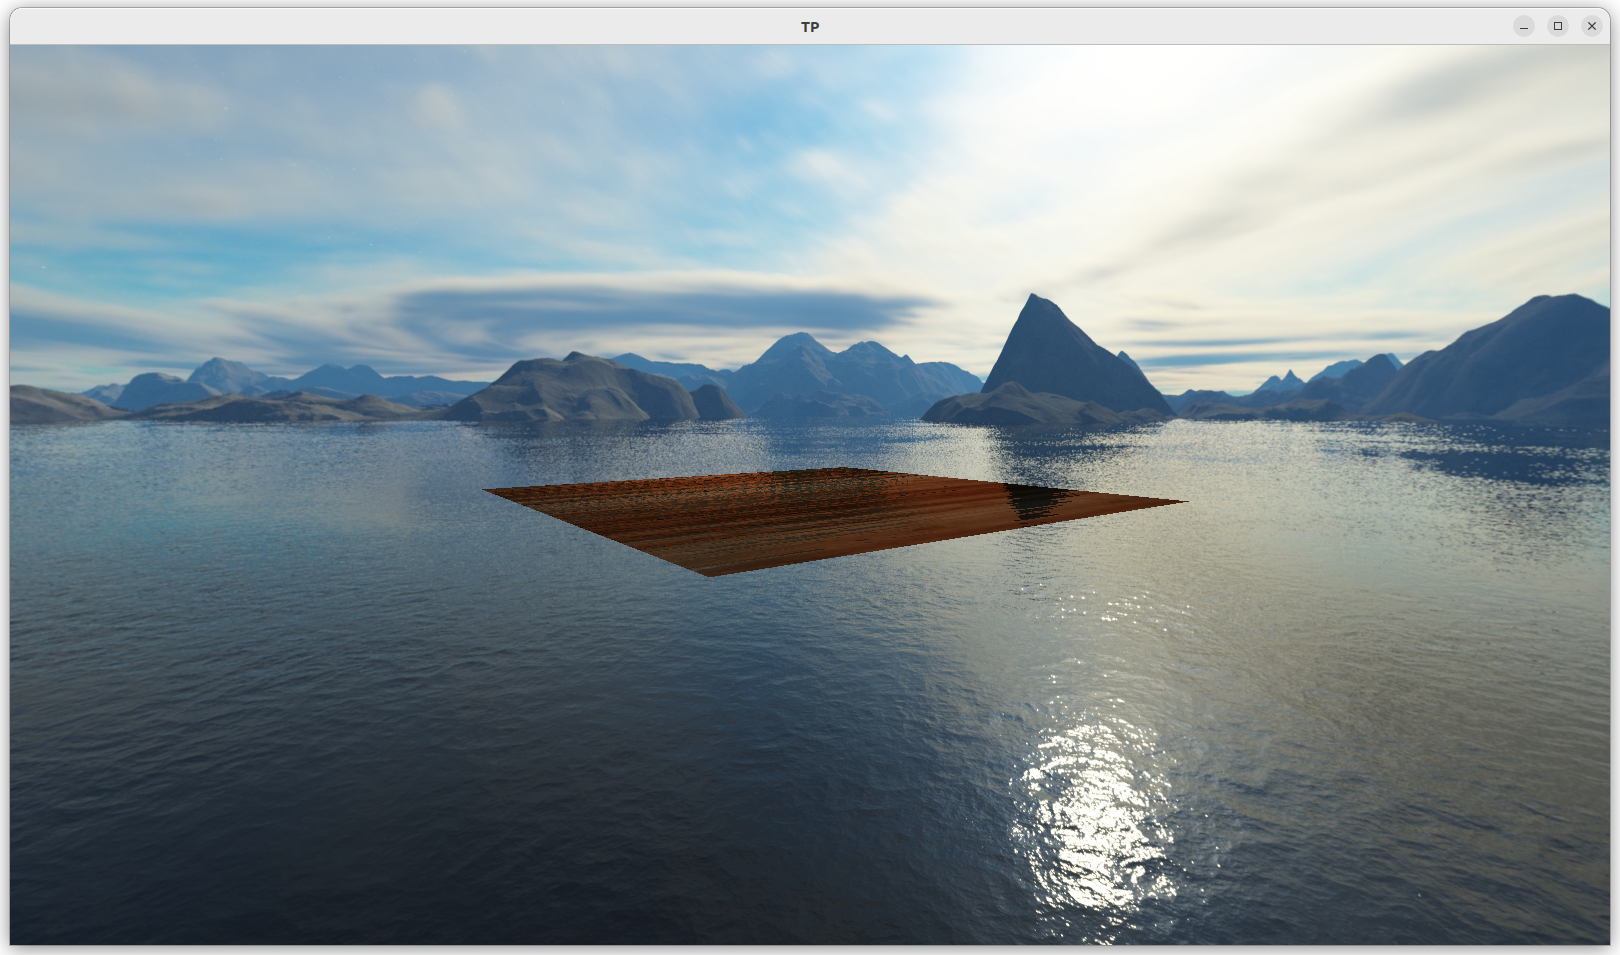
\includegraphics[width=\textwidth]{images/bizarrie1.png}
     \end{subfigure}
     \hfill
     \begin{subfigure}[b]{0.49\textwidth}
         \centering
         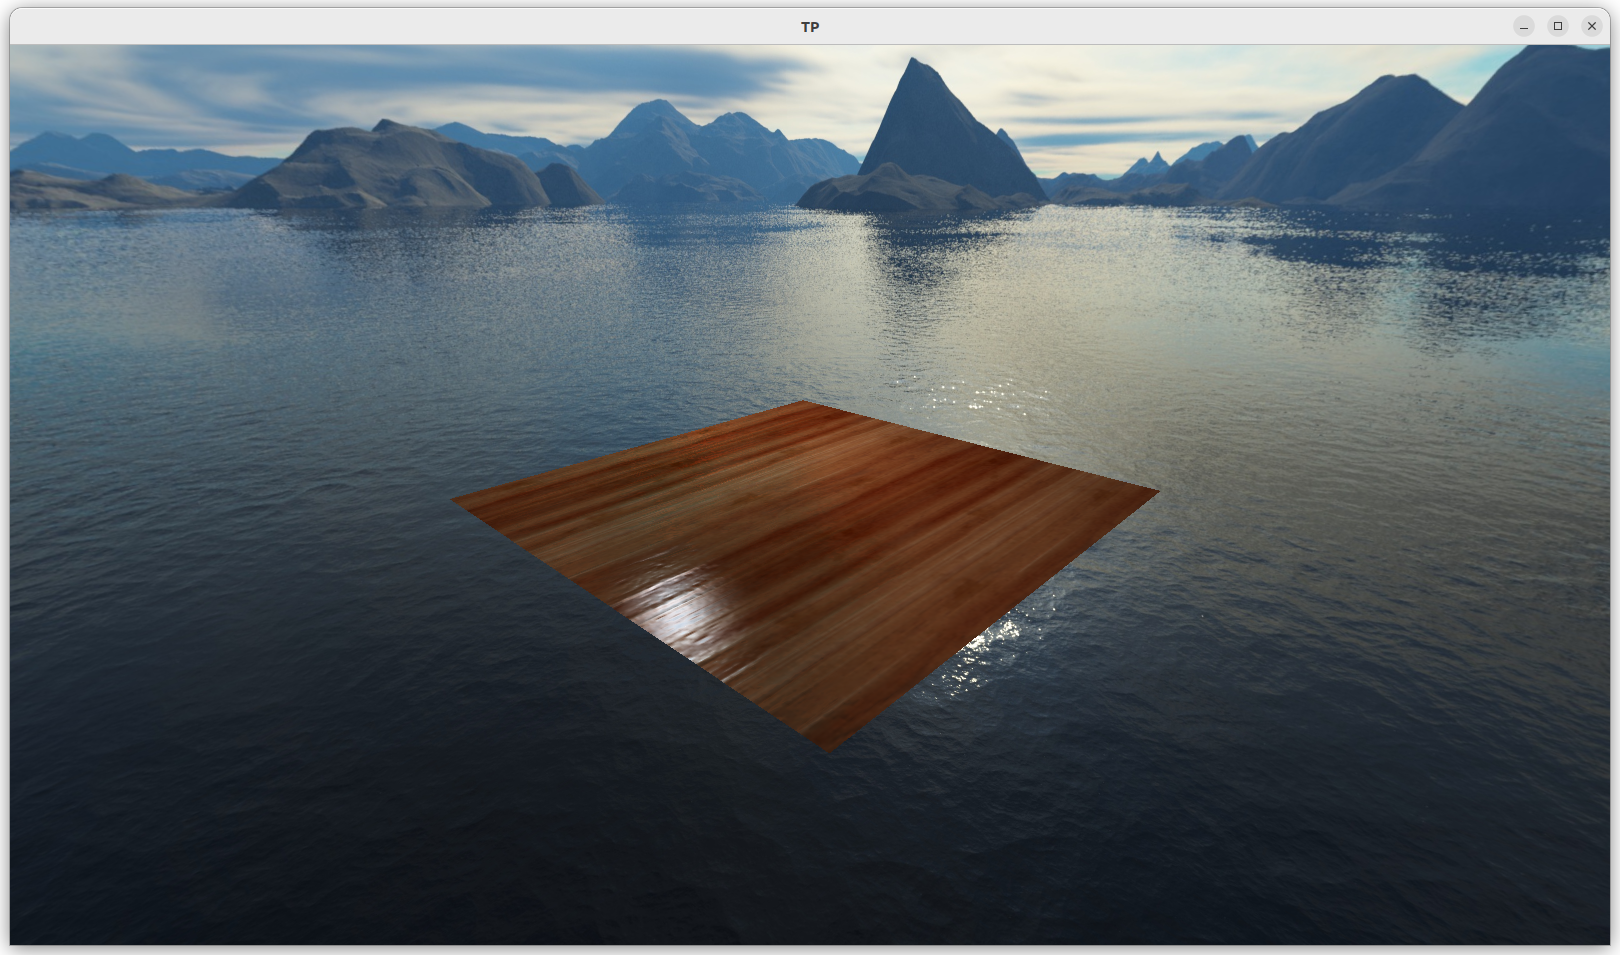
\includegraphics[width=\textwidth]{images/bizarrie2.png}
     \end{subfigure}
        \caption{Rendu reflectif + rendu reflectif avec couleur de l'objet}
        \label{fig:renduReflectif}
\end{figure}

\section{Liens}

Repo github : \url{https://github.com/Patateon/Prog-3D-TP4}

\end{document}